
% header %{{{1

\documentclass[tikz, border=1mm]{standalone}

\usepackage{amsmath}

\usepackage{tikz}

\usetikzlibrary{calc,angles,quotes,intersections,shapes.geometric}

\usepackage{tkz-euclide}

% document %{{{1

% opening %{{{2

\begin{document}

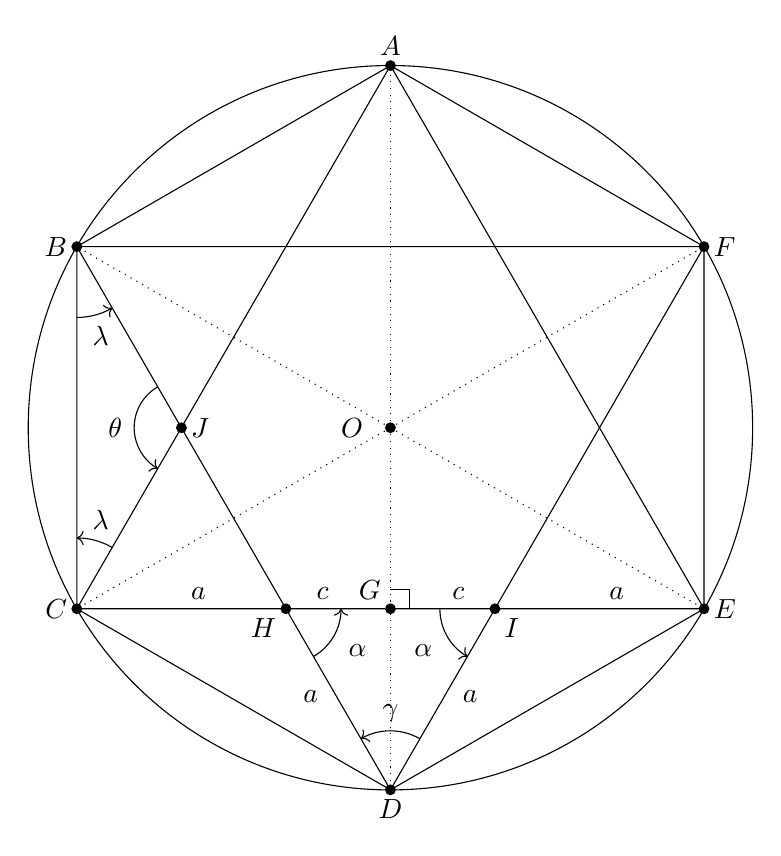
\begin{tikzpicture}[scale=2.3]

% parameters %{{{2

	\def\numsides{6}
	\def\radius{2}
	\def\rotation{90}

% coordinates %{{{2

	\coordinate (O) at (0,0);
	\foreach \i in {1,...,\numsides} {
		\coordinate (P\i) at ({360/\numsides*(\i-1)+\rotation}:\radius);
	}
	\coordinate (G) at (0,{-\radius/2});
	\coordinate (H) at ({-\radius*sqrt(3)/6},{-\radius/2});
	\coordinate (I) at ({\radius*sqrt(3)/6},{-\radius/2});

% intersections %{{{2

	%\path[name path=hexagram1] (P1) -- (P3);
	%\path[name path=hexagram2] (P2) -- (P4);
	%\path[name intersections={of=hexagram1 and hexagram2, by=J}];

	\tkzInterLL(P1,P3)(P2,P4)\tkzGetPoint{J}

% circle %{{{2

	\draw (O) circle (\radius);

% polygon %{{{2

	\draw (P1) \foreach \i in {2,...,\numsides} { -- (P\i) } -- cycle;

% radiuses %{{{2

	\foreach \i in {1,...,\numsides} { \draw[dotted] (O) -- (P\i); }

% hexagram %{{{2

	\draw (P1) -- (P3) -- (P5) -- cycle;
	\draw (P2) -- (P4) -- (P6) -- cycle;

% points, dots, vertices %{{{2

	\fill (O) circle (0.3mm);
	\fill (G) circle (0.3mm);
	\fill (H) circle (0.3mm);
	\fill (I) circle (0.3mm);
	\fill (J) circle (0.3mm);
	\foreach \i in {1,...,\numsides} { \fill (P\i) circle (0.3mm); }

% points, dots, vertices labels %{{{2

	\node[label={[label distance=1.0mm]left:$O$}] at (O) {};
	%\node[circle, fill, inner sep=1pt,
	%label={[label distance=2mm]left:$O$}] at (O) {};

	\node[above] at (P1) {$A$};
	\node[left] at (P2) {$B$};
	\node[left] at (P3) {$C$};
	\node[below] at (P4) {$D$};
	\node[right] at (P5) {$E$};
	\node[right] at (P6) {$F$};

	\node[above left] at (G) {$G$};
	\node[below left] at (H) {$H$};
	\node[below right] at (I) {$I$};
	\node[right] at (J) {$J$};

	\node[below left] at ($(H)!0.4!(P4)$) {$a$};
	\node[below right] at ($(I)!0.4!(P4)$) {$a$};
	\node[above right] at ($(P3)!0.5!(H)$) {$a$};
	\node[above right] at ($(H)!0.2!(G)$) {$c$};
	\node[above right] at ($(G)!0.5!(I)$) {$c$};
	\node[above right] at ($(I)!0.5!(P5)$) {$a$};

% angles labels %{{{

	\pic[draw, ->, "$\alpha$", angle radius=0.7cm, angle eccentricity=1.5]
	{angle = P4--H--G};

	\pic[draw, ->, "$\alpha$", angle radius=0.7cm, angle eccentricity=1.5]
	{angle = G--I--P4};

	\pic[draw, ->, "$\gamma$", angle radius=0.75cm, angle eccentricity=1.3]
	{angle = I--P4--H};

	\pic[draw, ->, "$\lambda$", angle radius=0.9cm, angle eccentricity=1.3]
	{angle = P3--P2--J};

	\pic[draw, ->, "$\lambda$", angle radius=0.9cm, angle eccentricity=1.3]
	{angle = J--P3--P2};

	\pic[draw, ->, "$\theta$", angle radius=0.6cm, angle eccentricity=1.4]
	{angle = P2--J--P3};

% right angles markers %{{{2

	\pic [draw, angle radius=7pt, angle eccentricity=1]
	{right angle = P5--G--O};

% closing %{{{2

\end{tikzpicture}
\end{document}
